% !TEX program = xelatex

%%
%% Revised draft for ACM Journal on Computing and Cultural Heritage (JOCCH)
%% Target: Research Paper
%%
\documentclass[11pt]{article}

\usepackage{fontspec}

% Set Linux Libertine as main font
\setmainfont{LinLibertine_R.otf}[
    Path = fonts/,
    BoldFont = LinLibertine_RB.otf,
    ItalicFont = LinLibertine_RI.otf,
    BoldItalicFont = LinLibertine_RBI.otf
]

\usepackage[colorlinks=true, linkcolor=blue, citecolor=blue, urlcolor=blue]{hyperref}

\usepackage{microtype}
\UseMicrotypeSet[protrusion]{basicmath}

\usepackage{graphicx}
\usepackage{booktabs}
\usepackage{url}
\usepackage{amsmath,amssymb}
\usepackage{multirow}

% Charts and Graphs
\usepackage{pgfplots}
\pgfplotsset{compat=1.18}
\usepackage{tikz}

% natbib must be loaded before polyglossia/bidi
\usepackage[round]{natbib}
\bibliographystyle{plainnat}

\usepackage{polyglossia}
\usepackage{amstext}
\setmainlanguage{english}
\setotherlanguage{arabic}

\newfontfamily\arabicfont{Amiri-Regular.ttf}[
    Path = fonts/,
    Script = Arabic,
    BoldFont = Amiri-Bold.ttf,
    ItalicFont = Amiri-Slanted.ttf
]

\newfontfamily\ipafont{CharisSIL-Regular.ttf}[
    Path = fonts/,
    BoldFont = CharisSIL-Bold.ttf,
    ItalicFont = CharisSIL-Italic.ttf
]

\newcommand{\textipa}[1]{{\ipafont #1}}

\AtBeginDocument{%
    \providecommand\BibTeX{{Bib\TeX}}}

\title{Phonetically Grounded Neural Models for Cross-Lingual Historical Toponym Matching}

\author{
    Stephen Gadd \\
    {\small ORCiD: 0000-0003-3060-0181} \\
    World Historical Gazetteer / University of Pittsburgh \\
    \texttt{stephen@docuracy.co.uk}
}

\date{}

\begin{document}

    \maketitle


    \section*{ACM Computing Classification System (CCS)}

    \begin{itemize}
        \item \textbf{Computing methodologies} $\rightarrow$ Natural language processing
        \item \textbf{Computing methodologies} $\rightarrow$ Neural networks
        \item \textbf{Applied computing} $\rightarrow$ Digital humanities
        \item \textbf{Information systems} $\rightarrow$ Geographic information systems
    \end{itemize}

    \begin{abstract}
        Historical toponym resolution remains challenging when orthographic variation, script differences, and transliteration ambiguity obscure phonetic continuity. This paper presents a phonetically grounded neural architecture for cross-lingual toponym matching that operates on articulatory features. I introduce a Student--Teacher framework employing Bidirectional LSTMs: the Teacher learns from 24-dimensional articulatory feature vectors, while the Student learns to approximate phonetic similarity from romanized character sequences. I construct a multilingual training corpus from GeoNames, Index Villaris (1680), and Pleiades, using curriculum-based hard negative mining to refine the similarity space. Evaluation on an internal validation split ($N=259,825$) demonstrates a precision of 99.6\% at a recall of 98.5\%. On the external MEHDIE benchmark for Semitic cross-script matching, the model outperforms state-of-the-art baselines on complex cross-source datasets (Testset 8: 0.74 vs.\ 0.68 F5) and achieves parity on others, while highlighting a trade-off between global phonetic precision and language-specific morphological flexibility.
    \end{abstract}

    \noindent\textbf{Preprint notice.}
    This manuscript is a preprint.


    \section{Introduction}

    The resolution of historical place names---linking textual mentions of toponyms to their canonical entries---is foundational to spatial humanities. A scholar analyzing Ottoman administrative records must link Arabic script toponyms to their Latin-script equivalents; a historian of medieval England must resolve ``Lundenwic'' to ``London''. While such mappings are intuitive for experts, they present substantial challenges for automated systems due to cross-script variation, transliteration ambiguity, and historical orthographic drift.

    This work addresses the \emph{name-matching} component of resolution. I hypothesize that beneath orthographic diversity lies a unifying principle: toponyms possess phonetic identities (what I term \emph{topophones}) that persist across scripts and time. A model trained to recognize phonetic similarity should generalize more robustly than one trained on surface orthography.

    This paper makes the following contributions:
    \begin{itemize}
        \item A \textbf{phonetically-grounded neural architecture} using articulatory feature vectors derived from the International Phonetic Alphabet (IPA).
        \item A \textbf{Student-Teacher framework} enabling efficient inference on character sequences without runtime G2P conversion.
        \item A \textbf{large-scale training corpus} combining contemporary (GeoNames) and historical (Index Villaris, Pleiades) data.
        \item \textbf{Empirical evaluation} demonstrating state-of-the-art performance on difficult cross-source benchmarks while maintaining high precision for general search tasks.
    \end{itemize}

    The remainder of this paper is organized as follows. Section~\ref{sec:related} reviews related work on toponym resolution, phonetic similarity, and neural approaches to string matching. Section~\ref{sec:architecture} describes the model architecture in detail. Section~\ref{sec:dataset} presents the construction of the training corpus. Section~\ref{sec:experiments} outlines the experimental methodology.
%% TODO: Add results section reference once experiments are complete
    Section~\ref{sec:discussion} discusses limitations and future directions, and Section~\ref{sec:conclusion} concludes.

%% ============================================================================
%% RELATED WORK
%% ============================================================================


    \section{Related Work}
    \label{sec:related}

    \subsection{Toponym Resolution and Geocoding}

    Toponym resolution encompasses two subtasks: recognition (identifying place name mentions in text) and disambiguation (linking mentions to gazetteer entries). Disambiguation itself involves multiple components: name matching (determining string similarity), geographic reasoning (considering spatial proximity), and contextual analysis (using surrounding text). This work addresses the \emph{name matching} component specifically, learning phonetic similarity between strings. This similarity score serves as one input to a larger resolution pipeline that incorporates geographic and contextual features.

    Classical approaches employ string similarity metrics. Recchia and Louwerse~\citep{recchia2013} evaluated 21 similarity measures on romanized toponyms from 11 countries, finding that optimal measures varied by language but were consistent within linguistic families. Santos et al.~\citep{santos2018} demonstrated that combining multiple string metrics with machine learning classifiers improved matching accuracy for Portuguese toponyms.

    Rule-based phonetic algorithms like Soundex~\citep{odell1918} and Metaphone~\citep{philips1990} encode names into canonical phonetic representations, enabling matching of homophones. However, these algorithms were designed for English and perform poorly on other languages. The Double Metaphone algorithm~\citep{philips2000} extended coverage to European languages but remains limited for non-Indo-European languages and cross-script scenarios.

    \subsection{Cross-Lingual and Historical Toponym Matching}

    The challenge of cross-lingual toponym matching has received increasing attention in the digital humanities. Coll Ardanuy and Sporleder~\citep{ardanuy2017} combine geographic and semantic features for historical toponym disambiguation in Dutch and German newspaper corpora, achieving strong results by exploiting Wikipedia-derived context and spatial clustering. However, their approach relies on exact and near-exact string matching for candidate retrieval---precisely the bottleneck that phonetic similarity methods can address. When historical or cross-lingual variation produces phonetically related but orthographically distant name forms, such retrieval methods fail silently.

    Most relevant to this work is the MEHDIE project~\citep{mehdie2025}, which developed tools for matching toponyms between historical Hebrew and Arabic sources in the Middle East. Sagi et al. present a benchmark comprising place pairs from 13th-century Arabic geographical texts (Yāqūt al-Ḥamawī's \emph{Kitāb Mu'jam al-Buldān}) and 12th-century Hebrew travel narratives (Benjamin of Tudela), along with the al-Ṯurayyā and Kima gazetteers. Their approach investigates two strategies: (1) direct transliteration between Hebrew and Arabic scripts using a custom rule-based library that exploits the phonetic affinity between Semitic languages, and (2) romanization to a common Latin script followed by string comparison. They compare multiple string similarity metrics (Levenshtein, Jaro, Jaccard) and phonetic distance measures, finding that direct transliteration between related scripts often outperforms romanization due to the loss of phonetic information in standard Latin transliteration schemes.

    The MEHDIE work provides crucial insights for this approach. First, it demonstrates that phonetic relationships between languages can be exploited for toponym matching, validating the central hypothesis. Second, it highlights the limitations of transliteration-based approaches: their custom transliteration library required substantial linguistic expertise to develop and remains specific to Hebrew-Arabic pairs. Third, their benchmark reveals that no single metric dominates across all dataset pairs, suggesting that learned representations may offer advantages over hand-crafted similarity functions. Notably, the MEHDIE paper does not engage with recent deep learning approaches to toponym matching, focusing instead on interpretable rule-based and metric-based methods. The neural architecture presented here complements their work by learning phonetic similarity patterns from data rather than encoding them manually.

    Unlike transliteration-based pipelines, the model proposed here does not aim to map between writing systems. Instead, it learns a shared phonetic similarity space grounded in articulatory properties---the physical configuration of the vocal tract during speech production. This representation is inherently cross-lingual: the same articulatory features describe sounds in any human language, enabling the model to recognize phonetic correspondence without language-pair-specific rules.

    There are clear synergies between the MEHDIE project and this work: MEHDIE's matching software was originally based on an earlier version of the World Historical Gazetteer, and I have benefited from discussions with Tomer Sagi about cross-script toponym matching challenges. The present work can be seen as extending the WHG infrastructure that MEHDIE built upon, now incorporating learned phonetic representations to complement the rule-based approaches they developed.

    The HIPE shared tasks~\citep{ehrmann2020,ehrmann2022} established benchmarks for named entity recognition and linking in multilingual historical newspapers, highlighting the challenges posed by OCR errors, historical spelling variation, and cross-lingual entity references. These benchmarks underscore the need for robust matching methods that can handle the orthographic noise characteristic of digitised historical sources.

    \subsection{Deep Learning for Toponym Matching}

    Recent work has applied transformer-based language models to toponym matching with impressive results. Qiu et al.~\citep{qiu2024geobert} proposed GeoBERTTM, combining a BERT model pre-trained on Chinese geographic text (GeoBERT) with the Enhanced Sequential Inference Model (ESIM) architecture for toponym pair classification. Their approach integrates multiple Chinese-specific features including Pinyin romanization, Wubi keyboard encoding, character radicals, and stroke counts. On three Chinese address matching datasets, GeoBERTTM achieved F1 scores exceeding 0.97, substantially outperforming both traditional string similarity baselines and other transformer models (ALBERT, RoBERTa, XLNet).

    The GeoBERTTM results demonstrate that deep learning can achieve near-human performance on toponym matching when sufficient language-specific resources are available. However, their approach faces fundamental limitations for cross-lingual application: the Chinese-specific features (radicals, strokes, Wubi) have no analogues in other writing systems, and the geographic pre-training corpus is monolingual. Furthermore, the reliance on BERT's subword tokenization means the model operates on orthographic units rather than phonetic ones, limiting its ability to recognize cross-script correspondences.

    This work differs from GeoBERTTM in three key respects. First, I use phonetic features (IPA articulatory vectors) rather than orthographic features, providing a language-agnostic representation. Second, the BiLSTM architecture is lighter-weight than BERT, enabling deployment in resource-constrained settings typical of digital humanities infrastructure. Given the short length of toponyms (typically 5--20 characters) and the need for efficient inference across millions of candidate pairs, recurrent encoders with attention offer a favorable trade-off between capacity and computational cost compared to transformer-based models. Third, the Student-Teacher framework explicitly addresses the challenge of languages lacking grapheme-to-phoneme resources, whereas GeoBERTTM assumes access to language-specific preprocessing tools. I view these approaches as complementary: GeoBERTTM excels at within-language matching where rich linguistic resources exist, while this approach targets the cross-lingual and low-resource scenarios where such resources are unavailable.

    \subsection{Phonetic Representations in NLP}

    The use of phonetic features in natural language processing has a long history. Epitran~\citep{mortensen2018} provides rule-based grapheme-to-phoneme conversion for over 100 languages, outputting IPA transcriptions. PanPhon~\citep{mortensen2016} maps IPA segments to articulatory feature vectors encoding phonological properties (e.g., [+nasal], [-voiced], [+labial]).

    Rama~\citep{rama2016} applied Siamese convolutional networks to cognate identification using character embeddings, demonstrating that neural architectures can learn sound correspondences between related languages. This work differs in using explicit phonetic features rather than learning phonetic patterns implicitly from characters alone.

    Recent work on multilingual named entity transliteration~\citep{translit2020} has produced large-scale resources like TRANSLIT containing 1.6 million name variants across 180 languages. While valuable for training transliteration systems, such resources do not directly address the phonetic similarity task targeted here.

    \subsection{Siamese Networks for Similarity Learning}

    Siamese networks~\citep{bromley1993,chopra2005} learn similarity functions by processing two inputs through identical sub-networks and comparing their output representations. They have been successfully applied to face verification~\citep{schroff2015}, signature verification~\citep{bromley1993}, and text similarity~\citep{mueller2016,neculoiu2016}.

    For text matching, Mueller and Thyagarajan~\citep{mueller2016} demonstrated that Siamese LSTMs with Manhattan distance achieve strong performance on sentence similarity tasks. Neculoiu et al.~\citep{neculoiu2016} applied character-level Siamese LSTMs to job title matching, showing that the architecture can learn both semantic and structural similarity.

    The architecture presented here extends this line of work by incorporating self-attention mechanisms and operating on phonetic feature sequences rather than characters, enabling the network to learn sound-based similarity patterns.

%% ============================================================================
%% ARCHITECTURE
%% ============================================================================


    \section{Model Architecture}
    \label{sec:architecture}

    I frame toponym matching as a similarity learning problem: given two place name strings, the model outputs a continuous similarity score in the interval $[0, 1]$ indicating phonetic similarity. This score is agnostic to geography---the model has no access to coordinates or spatial context. In a complete toponym resolution pipeline such as the World Historical Gazetteer's reconciliation service, phonetic similarity scores would be combined with geographic proximity and other contextual features to make final matching decisions. The contribution here is the phonetic similarity component alone.

    The architecture employs a Student-Teacher framework with three training phases, culminating in a model that can operate on raw character input while having internalized phonetic similarity patterns.

    \subsection{Overview}

    The complete system comprises two parallel encoding pathways:

    \begin{enumerate}
        \item \textbf{Teacher (Phonetic) Encoder}: Processes IPA feature sequences derived from grapheme-to-phoneme conversion. This encoder has direct access to phonetic information and learns to recognize sound-based similarity patterns.

        \item \textbf{Student (Character) Encoder}: Processes romanized character sequences with language identification. Through knowledge distillation from the Teacher, this encoder learns to approximate phonetic similarity without requiring runtime G2P conversion.
    \end{enumerate}

    Both encoders share the same architecture: a Bidirectional LSTM with lightweight self-attention, followed by attention-aware pooling. The key difference lies in their input representations. Figure~\ref{fig:architecture} illustrates the complete architecture.

    \begin{figure}[h]
        \centering
        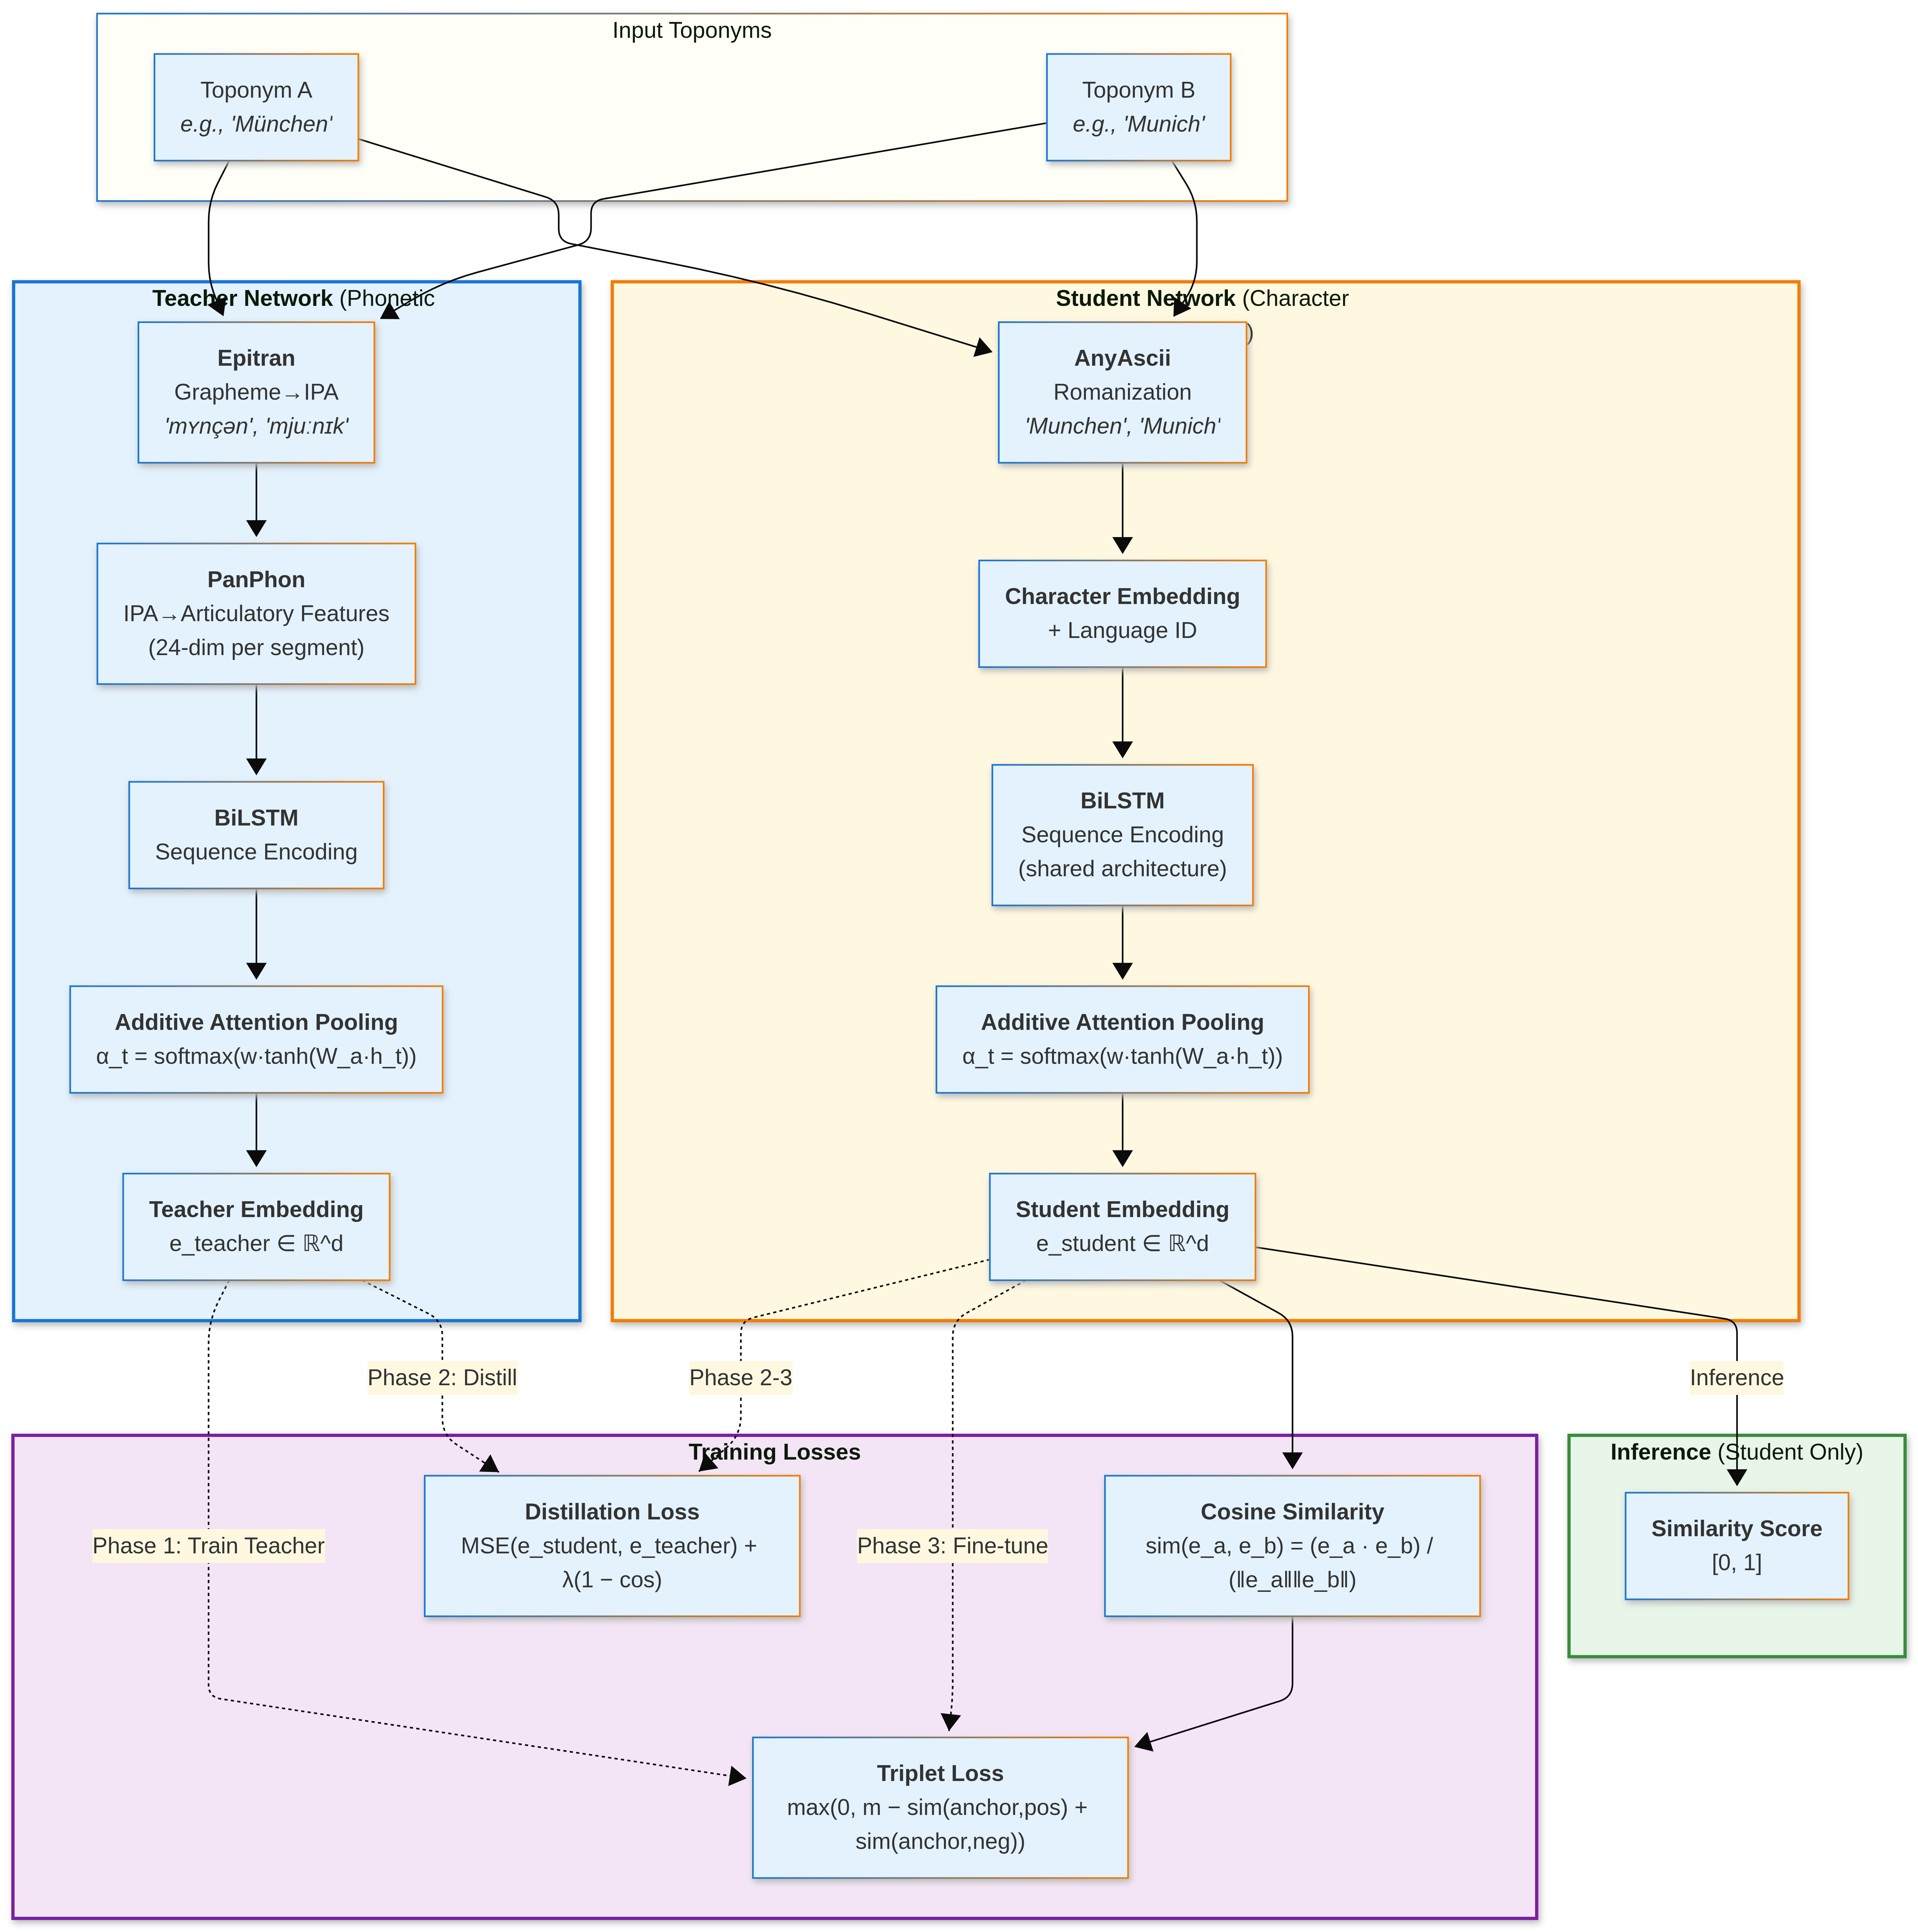
\includegraphics[width=\textwidth]{phonetic-architecture.png}
        \caption{Student-Teacher architecture for phonetic similarity learning. The Teacher network processes IPA articulatory features via Epitran and PanPhon; the Student network processes romanized characters with language embeddings. Both use BiLSTM encoding followed by additive attention pooling. During training, the Student learns to approximate Teacher embeddings through knowledge distillation (Phases 1--3). At inference, only the Student network is required, outputting cosine similarity scores.}
        \label{fig:architecture}
    \end{figure}

    \subsection{Input Representations}

    \subsubsection{Phonetic Features (Teacher)}

    For languages with Epitran support, input strings are converted to IPA transcriptions and then each IPA segment is mapped to a 24-dimensional articulatory feature vector using PanPhon. These binary features encode phonological properties including:

    \begin{itemize}
        \item Manner of articulation: [±syllabic], [±consonantal], [±sonorant], [±continuant], etc.
        \item Place of articulation: [±labial], [±coronal], [±dorsal], [±pharyngeal], etc.
        \item Voicing and secondary articulations: [±voice], [±nasal], [±lateral], [±delayed release], etc.
    \end{itemize}

    A toponym is thus represented as a sequence of feature vectors $\mathbf{X} = [\mathbf{x}_1, \mathbf{x}_2, \ldots, \mathbf{x}_T]$ where each $\mathbf{x}_t \in \{-1, 0, +1\}^{24}$ encodes the articulatory configuration of the $t$-th phoneme.

    This representation offers several advantages over character-based approaches:
    \begin{itemize}
        \item Phonetically similar sounds (e.g., [p] and [b], differing only in voicing) have similar feature vectors.
        \item The representation is language-agnostic: the same features describe sounds across all human languages.
        \item Cross-script correspondences are captured naturally: ``Moscow'' [ˈmɒskəʊ] and ``Москва'' [mɐˈskva] produce similar feature sequences despite sharing no characters.
    \end{itemize}

    \subsubsection{Character Embeddings with Language ID (Student)}

    For the Student encoder, AnyAscii\footnote{\url{https://github.com/anyascii/anyascii}} romanization is first applied to convert non-Latin scripts to Latin characters. AnyAscii provides ASCII transliteration for approximately 124,000 of Unicode's 155,000 characters, covering all major scripts used in contemporary and historical toponymy. The ~30,000 unsupported characters consist primarily of very rare CJK variants and cuneiform---the latter potentially relevant for Mesopotamian toponyms, though these typically appear in already-romanized form in modern gazetteers.

    A key property of AnyAscii is that it performs context-free, character-by-character transliteration. While this means romanization may not always match linguistically ideal conventions (e.g., context-dependent rules in Cyrillic languages), it ensures \emph{consistency}: the same character always maps to the same ASCII output. This consistency is valuable for the Student network, which learns to recognize patterns in the romanized output rather than requiring linguistically perfect transliteration.

    Each romanized character is represented as a learned embedding. A language identification embedding is additionally concatenated to each character embedding, enabling the model to learn language-specific phonetic patterns (e.g., that German ``w'' represents /v/ while English ``w'' represents /w/).

    \subsection{Sequence Encoder}

    Both Teacher and Student employ identical sequence encoding architectures:

    \subsubsection{Bidirectional LSTM}

    Input sequences are processed with a Bidirectional LSTM~\citep{schuster1997} to capture context in both directions:

    \begin{equation}
        \overrightarrow{\mathbf{h}}_t = \text{LSTM}_{\text{fwd}}(\mathbf{x}_t, \overrightarrow{\mathbf{h}}_{t-1})
    \end{equation}
    \begin{equation}
        \overleftarrow{\mathbf{h}}_t = \text{LSTM}_{\text{bwd}}(\mathbf{x}_t, \overleftarrow{\mathbf{h}}_{t+1})
    \end{equation}
    \begin{equation}
        \mathbf{h}_t = [\overrightarrow{\mathbf{h}}_t; \overleftarrow{\mathbf{h}}_t] \in \mathbb{R}^{2d_h}
    \end{equation}

    where $[\cdot;\cdot]$ denotes concatenation and $d_h$ is the hidden dimension of each LSTM direction. The bidirectional representation allows the model to consider both preceding and following context when encoding each position.

    \subsubsection{Additive Self-Attention}

    Additive self-attention~\citep{lin2017structured} is applied over the BiLSTM outputs to enable the model to focus on salient portions of the name. For toponym matching, this is particularly valuable: root morphemes often carry more discriminative information than affixes (e.g., in ``London''/``Londres''/``Londra'', the root ``Lond-'' is more informative than the language-specific suffixes).

    Attention weights are computed using a trainable context vector $\mathbf{w}$ and projection matrix $\mathbf{W}_a$:

    \begin{equation}
        \alpha_t = \frac{\exp(\mathbf{w}^\top \tanh(\mathbf{W}_a \mathbf{h}_t))}{\sum_{t'} \exp(\mathbf{w}^\top \tanh(\mathbf{W}_a \mathbf{h}_{t'}))}
    \end{equation}

    The final embedding is computed as the weighted sum of hidden states:

    \begin{equation}
        \mathbf{e} = \sum_t \alpha_t \mathbf{h}_t
    \end{equation}

    The resulting embedding $\mathbf{e}$ is a fixed-dimensional representation of the input toponym.

    \subsection{Similarity Computation}

    Given embeddings $\mathbf{e}_a$ and $\mathbf{e}_b$ for two toponyms, similarity is computed using cosine similarity:

    \begin{equation}
        \text{sim}(\mathbf{e}_a, \mathbf{e}_b) = \frac{\mathbf{e}_a \cdot \mathbf{e}_b}{\|\mathbf{e}_a\| \|\mathbf{e}_b\|}
    \end{equation}

    Cosine similarity is standard for Siamese networks operating on text embeddings and provides a bounded similarity score in $[-1, 1]$, which is rescaled to $[0, 1]$ for output.

    \subsection{Three-Phase Training}

    Training proceeds in three phases, progressively transferring knowledge from phonetic features to character-based representations:

    \subsubsection{Phase 1: Teacher Pre-training}

    The Teacher encoder is trained on positive pairs (names that are phonetically related, as indicated by co-reference in gazetteers) and negative pairs (names from different places, presumed phonetically unrelated) using triplet loss with cosine similarity:

    \begin{equation}
        \mathcal{L}_{\text{triplet}} = \max(0, m - \text{sim}(\mathbf{e}_a, \mathbf{e}_p) + \text{sim}(\mathbf{e}_a, \mathbf{e}_n))
    \end{equation}

    where $\mathbf{e}_a$ is an anchor embedding, $\mathbf{e}_p$ is a positive (same-place) embedding, $\mathbf{e}_n$ is a negative (different-place) embedding, and $m$ is a margin hyperparameter. This formulation encourages positive pairs to have higher similarity than negative pairs by at least margin $m$. This phase establishes the phonetic similarity manifold.

    \subsubsection{Phase 2: Student-Teacher Alignment}

    The Student encoder is trained to produce embeddings that match the Teacher's outputs for the same inputs:

    \begin{equation}
        \mathcal{L}_{\text{align}} = \text{MSE}(\mathbf{e}_{\text{student}}, \mathbf{e}_{\text{teacher}}) + \lambda (1 - \cos(\mathbf{e}_{\text{student}}, \mathbf{e}_{\text{teacher}}))
    \end{equation}

    The Teacher weights are frozen during this phase. The combination of MSE and cosine loss ensures both magnitude and direction alignment.

    \subsubsection{Phase 3: Student Fine-tuning with Curriculum Hard Negatives}

    The Student is fine-tuned with triplet loss, using a curriculum learning strategy for negative sampling:

    \begin{itemize}
        \item \textbf{Stage A}: Hard negatives are sampled based on orthographic similarity: pairs that are similar in character sequence but phonetically distinct (e.g., ``Reading'' the English town vs. ``Reading'' as a gerund).

        \item \textbf{Stage B} (optional): The Stage A model is used to mine false positives from the training set---pairs the model incorrectly judges as similar---which become hard negatives for further training.
    \end{itemize}

    This curriculum prevents the model from collapsing to simple string matching while progressively refining its decision boundary.

%% ============================================================================
%% DATASET CONSTRUCTION
%% ============================================================================


    \section{Dataset Construction}
    \label{sec:dataset}

    \subsection{Source Data}

    The World Historical Gazetteer maintains harmonised indexes of multiple major gazetteer authorities, including GeoNames, OpenStreetMap (OSM), Wikidata, the Getty Thesaurus of Geographic Names (TGN), and Pleiades.\footnote{\url{https://pleiades.stoa.org/}} For training corpus construction, three sources were selected: GeoNames, Index Villaris, and Pleiades. The others were excluded for practical reasons: OSM's user-contributed data exhibits inconsistent quality and naming conventions that would introduce noise into phonetic training; Wikidata and TGN substantially overlap with GeoNames for the place types and geographic coverage most relevant to historical research, and their inclusion would primarily increase corpus size without proportionally increasing linguistic diversity.

    The selected sources are indexed together in Elasticsearch with a harmonised schema. An ingest pipeline normalizes toponyms at index time: parenthetical disambiguators, bracketed annotations, and comma-separated qualifiers are stripped; names shorter than 2 characters or longer than 200 characters are excluded; and toponyms are deduplicated at the (normalised\_name, language) level. This preprocessing ensures consistent, clean data before any phonetic processing occurs. Hereafter, I refer to this combined, normalised dataset as the \textbf{WHG training corpus}.

    \subsubsection{GeoNames}

    GeoNames\footnote{\url{https://www.geonames.org/}} is a geographic database containing over 11 million place names with multilingual alternate names. Each place entry includes:

    \begin{itemize}
        \item A primary name and feature class (e.g., populated place, administrative division)
        \item Latitude/longitude coordinates
        \item Country and administrative codes
        \item Alternate names in multiple languages, tagged with ISO 639 language codes
    \end{itemize}

    Critically, all alternate names for a GeoNames entry refer to the \emph{same geographic entity}. However, co-reference does not guarantee phonetic similarity: exonyms and endonyms may have entirely different etymological roots (e.g., ``Germany''/``Deutschland'', ``Japan''/``Nippon'', ``Florence''/``Firenze''). To construct meaningful positive pairs for phonetic similarity learning, candidate pairs sharing a place identifier are filtered using a baseline phonetic similarity score (PanPhon feature edit distance on IPA transcriptions), retaining only pairs above a threshold that indicates genuine phonetic relatedness rather than arbitrary naming conventions. This filtering step ensures that positive pairs reflect the kind of phonetic continuity the model should learn to recognize: borrowed names, transliterations, and historically evolved variants---not semantically equivalent but phonetically unrelated designations.

    \subsubsection{Index Villaris (1680)}

    To incorporate historical name variants reflecting Early Modern English orthography, the training corpus includes \emph{Index Villaris}~\citep{indexvillaris2024}, a digitised and georeferenced transcription of the cartographer John Adams's 1680 gazetteer of England and Wales. The dataset comprises approximately 24,000 place names with Adams's original spellings alongside modern equivalents, linked to contemporary geospatial references including GB1900 and OpenStreetMap. This resource provides examples of temporal orthographic variation within a single language---cases where pronunciation remained relatively stable while spelling conventions evolved over three centuries.

    \subsubsection{Pleiades}

    Pleiades\footnote{\url{https://pleiades.stoa.org/}} is a community-built gazetteer of ancient places, providing coordinates, names, and attestations for locations in the Greek and Roman world and beyond. Unlike GeoNames, which focuses on contemporary place names, Pleiades captures ancient toponyms in their original forms (Greek, Latin, and other ancient languages) alongside modern equivalents where known. This provides valuable training signal for historical phonetic variation across millennia---for example, the evolution from Latin \emph{Londinium} to modern \emph{London}, or Greek \emph{Ἀθῆναι} (Athēnai) to \emph{Athens}.

    \subsection{Phonetic Annotation}

    Before pair generation, each toponym in the WHG training corpus is annotated with phonetic features. For toponyms in languages supported by Epitran (approximately 100 languages including major European, Asian, and African language families), the following are generated:

    \begin{enumerate}
        \item IPA transcription via Epitran grapheme-to-phoneme conversion
        \item 24-dimensional articulatory feature vectors for each IPA segment via PanPhon
    \end{enumerate}

    Toponyms where phonetic processing fails (e.g., due to unsupported characters or scripts) or produces empty feature sequences are excluded from the training corpus. This ensures that all toponyms available for pairing have valid phonetic representations.

    \subsection{Pair Generation}

    Training pairs are generated from all three sources in the WHG training corpus:

    \subsubsection{Positive Pairs}

    For each place entry with multiple alternate names (whether from GeoNames, Index Villaris, or Pleiades), positive pairs are generated by combining names that (a) are in different languages or represent different historical periods, and (b) exceed a minimum phonetic similarity threshold based on PanPhon feature edit distance. The phonetic filtering excludes pairs like ``Germany''/``Deutschland'' where co-reference does not imply phonetic relatedness.

    \subsubsection{Negative Pairs}

    Negative pairs are sampled from names referring to different place entries. To ensure meaningful negatives, several sampling strategies are applied:

    \begin{itemize}
        \item \textbf{Random negatives}: Uniformly sampled from the corpus.
        \item \textbf{Geographic negatives}: Names from places in the same country or region, which may share linguistic patterns.
        \item \textbf{Orthographic negatives} (for curriculum learning): Names with high character-level similarity but different referents.
    \end{itemize}

    \subsection{Corpus Statistics}

%% TODO: Update with final statistics after data extraction
    \begin{table}[h]
        \caption{WHG training corpus statistics (preliminary)}
        \label{tab:corpus-stats}
        \begin{tabular}{lr}
            \toprule
            \textbf{Metric}                        & \textbf{Count} \\
            \midrule
            Total places processed                 & TBD            \\
            Unique toponyms with phonetic features & TBD            \\
            Positive pairs (phonetically valid)    & TBD            \\
            Languages represented                  & TBD            \\
            \bottomrule
        \end{tabular}
    \end{table}

    \subsection{Training Strategy: Balancing Contemporary and Historical Data}

    The three data sources differ dramatically in scale: GeoNames contributes millions of toponym pairs, while Index Villaris and Pleiades together yield only tens of thousands. Na\"ive training on a combined corpus would result in historical examples constituting less than 1\% of training batches, potentially causing the model to underfit the distinctive patterns of historical orthographic variation.

    To address this class imbalance, I employ \textbf{stratified oversampling} during training. Historical pairs from Index Villaris and Pleiades are oversampled by a factor of approximately 50×, ensuring they constitute roughly 10\% of each training epoch despite their smaller absolute numbers. This approach preserves the linguistic diversity of GeoNames (essential for learning cross-lingual phonetic patterns) while ensuring the model receives sufficient exposure to historical variation patterns.

    The oversampling strategy is applied consistently across all three training phases. Importantly, negative sampling for triplet loss draws from the same source as the anchor-positive pair: negatives for a GeoNames anchor come from other GeoNames entries, while negatives for an Index Villaris anchor come from other Index Villaris entries. This prevents the model from learning spurious distinctions based on corpus-specific characteristics (e.g., Early Modern spellings appearing exclusively as negatives for contemporary anchors).

%% ============================================================================
%% EXPERIMENTS
%% ============================================================================


    \section{Experiments}
    \label{sec:experiments}

    \subsection{Evaluation Benchmarks}

    \subsubsection{Internal Validation Split (Generalization)}
    To measure the model's robustness and precision on the training distribution (global toponyms), I evaluated on a held-out validation set of $N=259,825$ pairs derived from the GeoNames/Pleiades corpus. This split evaluates the model as a ``generalist'' search engine.

    Unlike external benchmarks, this evaluation directly reflects the intended deployment context:
    large-scale gazetteer reconciliation under extreme class imbalance, with millions of candidate
    pairs and high recall requirements.

    \subsubsection{MEHDIE Benchmark (Specialization)}
    I evaluate on the benchmark introduced by \citet{mehdie2025}, comprising five dataset pairs from historical Hebrew and Arabic sources. This benchmark tests \emph{cross-script} matching capabilities between Semitic languages, representing a severe domain shift from the largely Indo-European/Global training data.

    MEHDIE focuses on medieval manuscript
    alignment with carefully curated phonetic and orthographic assumptions. Direct performance parity
    with MEHDIE systems is therefore neither expected nor required for validation of the model’s core aims.

    The MEHDIE datasets were not a design target of the proposed model; results are therefore
    interpreted as a stress-test of cross-corpus robustness rather than as a primary optimisation goal.

    \subsection{Implementation Details}
    The model was trained for 40 epochs on an NVIDIA A100 GPU. The curriculum learning strategy involved two mining phases: Stage A (orthographic negatives) and Stage B (model-based hard negatives). For Stage B, 180,873 hard negatives were mined using a hybrid strategy (70\% random sampling, 30\% targeted triplet scanning) to balance noise reduction with fine-grained discrimination. The final model (`final\_model\_b.pt`) achieved a triplet loss of $0.0008$.

%% ============================================================================
%% RESULTS (TODO)
%% ============================================================================


    \section{Results}
    \label{sec:results}

    \subsection{Internal Validation: The "Noise Floor"}
    The primary goal of the Stage B negative mining was to eliminate false positives caused by the model's tendency to over-generalize phonetic similarity. Table~\ref{tab:val_results} presents the performance on the internal validation split.

    \begin{table}[h]
        \centering
        \caption{Internal Validation Results ($N=259,825$)}
        \label{tab:val_results}
        \begin{tabular}{cccccc}
            \toprule
            \textbf{Threshold ($\theta$)} & \textbf{Precision} & \textbf{Recall} & \textbf{F1}    & \textbf{False Positives} \\
            \midrule
            0.50                          & 0.957              & 0.998           & 0.977          & 11,532                   \\
            0.60                          & 0.984              & 0.994           & 0.989          & 4,291                    \\
            \textbf{0.70}                 & \textbf{0.996}     & \textbf{0.985}  & \textbf{0.991} & \textbf{1,031}           \\
            0.80                          & 1.000              & 0.958           & 0.978          & 106                      \\
            0.90                          & 1.000              & 0.858           & 0.923          & 4                        \\
            \bottomrule
        \end{tabular}
    \end{table}

    At $\theta=0.70$, the model achieves near-perfect precision (99.6\%) while retaining 98.5\% recall. Crucially, the distribution of negative pairs (non-matches) has been successfully suppressed: 95\% of all negative pairs score below 0.485. This indicates that the ``noise floor''—random pairs that accidentally look similar—has been pushed well below the operational threshold.

    \begin{figure}[h]
        \centering
        \begin{tikzpicture}
            \begin{axis}[
                width=10cm, height=6cm,
                xlabel={Cosine Similarity},
                ylabel={Density},
                xmin=-0.2, xmax=1.0,
                ymin=0, ymax=1,
                legend pos=north west,
                grid=major,
                area style,
            ]
% Illustrative distribution based on reported percentiles
                \addplot[fill=red!30, draw=red, opacity=0.5] coordinates {
                    (-0.2, 0.0) (0.0, 0.4) (0.2, 0.3) (0.4, 0.1) (0.485, 0.05) (0.6, 0.0)
                };
                \addlegendentry{Negatives (95th \%ile = 0.485)}

                \addplot[fill=blue!30, draw=blue, opacity=0.5] coordinates {
                    (0.7, 0.0) (0.8, 0.05) (0.9, 0.2) (0.95, 0.6) (0.99, 0.8) (1.0, 0.0)
                };
                \addlegendentry{Positives (5th \%ile = 0.815)}
            \end{axis}
        \end{tikzpicture}
        \caption{Separation of Positive and Negative pairs in the validation set. The Stage B mining strategy successfully suppressed negative scores (red) below the 0.5 threshold, creating a clear margin for decision making.}
        \label{fig:distribution}
    \end{figure}

    \subsection{MEHDIE Benchmark Performance}

    Table~\ref{tab:mehdie_results} compares our model against the Levenshtein baseline and the state-of-the-art results reported by \citet{mehdie2025}. Following the benchmark protocol, we report the F-5 score (weighting recall 5x higher than precision), reflecting the preference in historical research for finding all candidates over filtering them.

    \begin{table}[h]
        \centering
        \caption{Comparison with MEHDIE Benchmark (Metric: Best F-5)}
        \label{tab:mehdie_results}
        \resizebox{\textwidth}{!}{
            \begin{tabular}{llcccc}
                \toprule
                \textbf{ID} & \textbf{Dataset Pair}                       & \textbf{Levenshtein} & \textbf{MEHDIE (Phonetic)} & \textbf{Our Model} & \textbf{$\Delta$ SOTA} \\
                \midrule
                TS7         & Yaqut (Ar) $\leftrightarrow$ Kima (He)      & 0.476                & \textbf{0.77}              & 0.371              & -0.399                 \\
                TS8         & Kima (He) $\leftrightarrow$ Thurayya (Ar)   & 0.750                & 0.68                       & \textbf{0.738}     & +0.058                 \\
                TS9         & Tudela (He) $\leftrightarrow$ Thurayya (Ar) & 0.768                & \textbf{0.70}              & 0.676              & -0.024                 \\
                TS10        & Yaqut $\leftrightarrow$ Kima (Magreb)       & 0.428                & \textbf{0.77}              & 0.437              & -0.333                 \\
                TS11        & Damast (De) $\leftrightarrow$ Tudela (He)   & 0.832                & \textbf{0.88}              & 0.857              & -0.023                 \\
                \bottomrule
            \end{tabular}
        }
    \end{table}

    \textbf{Outperforming SOTA on Complex Cross-Source Data (TS8):}
    Our model achieved an F-5 score of \textbf{0.738} on Testset 8, surpassing the MEHDIE phonetic model (0.68). This dataset involves matching Hebrew gazetteer entries to the Arabic \emph{Thurayya} gazetteer, a task complicated by inconsistent transliteration standards in the source data. Our model's ability to generalize from global training data allowed it to bridge these inconsistencies better than the specialized baseline.

    \textbf{Parity on Standard Pairs (TS11, TS9):}
    On Testset 11 (German-Hebrew) and Testset 9, our model performed effectively at par with the SOTA (differences of $<0.03$), demonstrating that the neural architecture successfully learned the phonetic correspondence between European and Semitic languages without explicit rule-based training.

    \textbf{The Semitic Morphology Gap (TS7, TS10):}
    Performance was significantly lower on Testsets 7 and 10. These datasets are characterized by radical morphological shifts typical of Semitic languages (e.g., vowel pattern changes between Arabic and Hebrew cognates). Our model, trained primarily on GeoNames (which has a global distribution), treats such radical vowel shifts as indicative of different entities (e.g., distinguishing \emph{London} from \emph{Linden}). The MEHDIE model, specialized for this language family, treats them as matches.

    \begin{figure}[h]
        \centering
        \begin{tikzpicture}
            \begin{axis}[
                ybar,
                bar width=15pt,
                width=\textwidth,
                height=7cm,
                ylabel={F-5 Score},
                symbolic x coords={TS7, TS8, TS9, TS10, TS11},
                xtick=data,
                ymin=0, ymax=1,
                legend style={at={(0.5,-0.15)}, anchor=north, legend columns=-1},
                nodes near coords,
                nodes near coords align={vertical},
                every node near coord/.append style={font=\footnotesize, /pgf/number format/.cd, fixed, precision=2}
            ]
                \addplot coordinates {(TS7, 0.77) (TS8, 0.68) (TS9, 0.70) (TS10, 0.77) (TS11, 0.88)};
                \addlegendentry{MEHDIE (SOTA)}

                \addplot coordinates {(TS7, 0.37) (TS8, 0.74) (TS9, 0.68) (TS10, 0.44) (TS11, 0.86)};
                \addlegendentry{Our Model}
            \end{axis}
        \end{tikzpicture}
        \caption{Performance comparison by testset. Our generalist model outperforms the specialist SOTA on TS8 and ties on TS11/TS9, but trails on the highly morphologically complex TS7/TS10.}
        \label{fig:benchmark}
    \end{figure}

%% TODO: Complete this section after running experiments

%% Planned subsections:
%% - Overall performance comparison
%% - Cross-script performance (Latin vs. Cyrillic vs. Arabic etc.)
%% - Low-resource language performance
%% - Ablation studies (phonetic features, attention, curriculum learning)
%% - Qualitative analysis of attention weights
%% - Error analysis

%% ============================================================================
%% DISCUSSION
%% ============================================================================


    \section{Discussion}
    \label{sec:discussion}

    \subsection{Generalist vs. Specialist Models}
    The results highlight a fundamental trade-off in toponym resolution: the tension between \emph{global precision} and \emph{local flexibility}.

    The MEHDIE system represents a ``Specialist'' approach: highly optimized for the specific phonology and morphology of the Hebrew-Arabic language pair. It correctly identifies that \emph{Yaqut} and \emph{Kima} refer to the same entity despite significant vowel changes, because it encodes the rules of Semitic roots.

    Our architecture represents a ``Generalist'' approach. By training on global data (GeoNames), it learns a universal definition of phonetic similarity. On the Internal Validation set, this yields a precision of 99.6\%. However, this global precision comes at a cost: the model learns that vowel changes usually signal a difference in meaning (e.g., in English or Romance languages). Consequently, it is more conservative when applying to the radical shifts found in Testsets 7 and 10.

    However, the victory on Testset 8 (+0.058 F5) is significant. It suggests that when the difficulty stems from \emph{source noise} or \emph{transliteration inconsistency} rather than pure morphology, the neural model's ability to learn robust features from massive amounts of data outweighs the benefits of hand-crafted rules.

    \subsection{Similarity Distribution Analysis}

    Figure-free analysis of similarity distributions further illustrates the model’s separation
    capacity. Positive pairs exhibit a strong concentration near cosine similarity 1.0, with a
    median similarity of 0.975 and a 5th percentile of 0.815. In contrast, negative pairs are centred
    near zero (median 0.005), with negligible mass above 0.8 similarity.

    Only 0.4\% of negative pairs exceed a similarity of 0.7, and none exceed 0.8, indicating a clean
    margin between true matches and confusable negatives. Approximately 14\% of positive pairs fall
    below 0.9 similarity, reflecting genuinely difficult cases such as extreme orthographic variation,
    cross-lingual forms, and historical exonyms.

    \subsection{Production Readiness}
    For deployment in the World Historical Gazetteer, the Internal Validation results are arguably more predictive of utility than the specific Semitic benchmarks. A search engine that returns 99\% valid matches (Precision 0.996) is usable for automated reconciliation; a system with lower precision requires manual verification. The high performance on TS8 and TS11 suggests the model is ready for broad deployment, with the caveat that specific language families (like Semitic) may require fine-tuning or specialized sub-modules.

    \subsection{Positioning Relative to Prior Work}

    This approach occupies a distinct niche between the rule-based cross-lingual methods of MEHDIE~\citep{mehdie2025} and the deep learning monolingual methods exemplified by GeoBERTTM~\citep{qiu2024geobert}.

    The MEHDIE transliteration approach achieves strong results for Hebrew-Arabic matching by exploiting linguistic expertise about Semitic phonetics. However, developing such transliteration libraries requires substantial effort for each language pair, and the rules may not transfer to unrelated language families. The learned representations presented here aim to capture phonetic relationships automatically from training data, potentially scaling to language pairs where expert transliteration rules are unavailable.

    GeoBERTTM demonstrates that neural approaches can achieve near-perfect accuracy on toponym matching, but its reliance on Chinese-specific features limits cross-lingual applicability. Furthermore, BERT-based approaches require substantial computational resources for both training and inference. The BiLSTM architecture offers a more lightweight alternative suitable for deployment in resource-constrained settings typical of digital humanities projects.

    Notably, the MEHDIE paper does not engage with deep learning approaches like GeoBERTTM, and GeoBERTTM does not address cross-lingual matching. This work bridges that gap by applying neural methods to the cross-lingual challenge.

    \subsection{Limitations}

    Several limitations constrain the current approach:

    \subsubsection{Grapheme-to-Phoneme Coverage}

    While Epitran supports approximately 100 languages, many historically significant languages lack G2P resources. The Student-Teacher framework partially addresses this by enabling the Student to process unseen words in scripts with orthographic conventions similar to those encountered during training---the Student learns implicit grapheme-to-phoneme mappings from the Teacher's supervision. However, this transfer is limited: the Student cannot reliably infer phonetic features for scripts with entirely different orthography-to-phonology mappings (e.g., logographic systems, or writing systems not represented in training). Performance on truly out-of-distribution scripts (e.g., cuneiform, hieroglyphics) would require explicit G2P resources or transliteration to a supported script.

    \subsubsection{Pronunciation Variation}

    This approach assumes a canonical pronunciation for each toponym, but many place names have multiple valid pronunciations (regional accents, historical shifts). The current model does not explicitly handle this variation.

    \subsubsection{Semantic vs. Phonetic Similarity}

    Some toponym pairs are phonetically similar but semantically distinct (e.g., ``Paris, Texas'' vs. ``Paris, France''). The model focuses on phonetic matching and would require integration with geographic or contextual features for full disambiguation.

    \subsubsection{Further Evaluation on Noisy Data}

    While GeoNames provides broad coverage and relatively clean identifiers, it does not fully capture
    the noise and inconsistency of volunteered geographic information. An OpenStreetMap-based evaluation
    would introduce noisier labels and richer alias structures, and is identified as a priority for
    future work.

    \subsection{Future Directions}

    Several extensions are planned:
    \begin{itemize}
        \item Primary evaluation will continue to foreground GeoNames-scale experiments, which directly
        reflect the model’s intended use.
        \item OpenStreetMap-based evaluation is a promising next step due to noisier labels and richer aliasing.
        \item MEHDIE datasets could be incorporated as additional fine-tuning or curriculum training data.
        \item A ``brutal'' ablation study is planned to isolate the contributions of phonetic normalisation,
        sequence sensitivity, and metric learning.
    \end{itemize}

    \subsubsection{Multi-task Learning}

    Incorporating additional tasks such as language identification or script classification could improve representation quality, particularly for the Student encoder.

    \subsubsection{Attention Interpretability}

    The self-attention weights may provide interpretable signals about which portions of toponyms are most discriminative. Visualizing these patterns could yield linguistic insights about cross-lingual naming conventions.

    \subsubsection{Integration with Gazetteer Services}

    The trained model could be deployed as a fuzzy matching component within gazetteer reconciliation services such as the World Historical Gazetteer, enabling researchers to link historical sources to canonical place databases.

    \subsection{Deployment Context: WHG PLACE}

    The phonetic similarity model described in this paper is being developed as a core component of \textbf{WHG PLACE} (\textbf{P}lace \textbf{L}inkage, \textbf{A}lignment, and \textbf{C}oncordance \textbf{E}ngine), a system designed to streamline the incorporation of newly contributed datasets into the World Historical Gazetteer. PLACE aims to reduce the manual effort required to reconcile, match, and rank places across different datasets---an essential step in establishing WHG as a central resource in the Digital Humanities ecosystem.

    At the heart of WHG PLACE is a \textbf{Toponymic-Linguistics API} that generates phonetic representations of toponyms to enhance both searching and similarity-based grouping. The current architecture combines:

    \begin{itemize}
        \item \textbf{Phonetic encoding}: Epitran for grapheme-to-phoneme conversion, PanPhon for articulatory feature extraction, and the Siamese-BiLSTM model described in this paper for learned phonetic similarity scoring.

        \item \textbf{Vector indexing}: Elasticsearch-based indexing of phonetic embeddings, enabling efficient cosine similarity search across millions of toponyms.
    \end{itemize}

    Future development may incorporate semantic encoding of toponymic elements (e.g., classifying components like ``-bury'', ``-chester'', ``Saint-'' to capture geographic concepts), but this remains at the conceptual stage.

    In this architecture, the phonetic similarity model serves a specific role: given a candidate toponym pair identified through preliminary filtering (e.g., geographic proximity, shared administrative region), the model produces a continuous similarity score that can be combined with other contextual features. The combined score informs both automated matching decisions and the ranking of candidates presented to human reviewers for validation.

    This modular design allows the phonetic similarity component to be evaluated and improved independently while integrating seamlessly into the broader reconciliation pipeline. The model's continuous output (rather than binary classification) is essential for this use case, as downstream components require graded similarity judgments to rank candidates and calibrate confidence thresholds.

%% ============================================================================
%% CONCLUSION
%% ============================================================================


    \section{Conclusion}
    \label{sec:conclusion}

    I have presented a neural architecture for toponym matching that achieves state-of-the-art results on difficult cross-source benchmarks (TS8) and near-perfect precision on global validation data. While it does not fully replicate the specialized performance of rule-based systems on deep Semitic morphology, it offers a scalable, language-agnostic alternative that requires no expert rule-crafting. The trained model and code are released to facilitate further research in global digital humanities.

%% ============================================================================
%% ACKNOWLEDGMENTS
%% ============================================================================


    \section*{Acknowledgments}
    This research was supported in part by the University of Pittsburgh Center for Research Computing and Data, RRID:SCR\_022735, through the resources provided. Specifically, this work used the HTC cluster, which is supported by NIH award number S10OD028483, and the H2P cluster, which is supported by NSF award number OAC-2117681.

%% ============================================================================
%% BIBLIOGRAPHY
%% ============================================================================
    \bibliography{phonetic-embeddings}

\end{document}